%Chapter 2 - Literature Review

\chapter{Literature Review} % Main chapter title
\label{Chapter2} % For referencing the chapter elsewhere, use \ref{Chapter2} 

%----------------------------------------------------------------------------------------
%----------------------------------------------------------------------------------------
\section{Early home computer era} \label{sec: Early home computer era}
 
The mid-1970s to late-1980s was an interesting period in the history of computers. It marked the first time computers were designed and marketed for personal use in the home; the early home computer era. The term \textit{home computer} is ambiguous and not defined by any standard. In this thesis it is taken to be synonymous with a microcomputer or a personal computer (PC) from the era. A PC is classified in the \textit{Proceedings of the IEEE} from 1984 by Gupta, A. and Toong, H. as a computer that fulfils all of the following characteristics 
\cite{RN24}: 

\begin{enumerate}
\item The computer cost less than \$5000 USD at the time of sale.
\item The computing power is provided by a microprocessor from the era. 
\item The computer is sold through mass-marketing channels. 
\item The computer can run a variety of programs for different fields such as industry, business, education and at home; it is a general purpose computer, not designed for a single purpose or a single type of user.
\item The computer can handle at least one high-level language such as BASIC, FORTRAN, or COBOL.
\end{enumerate}

Since the discovery of semiconductors in the 1940s, there have been continuous efforts and advances in making electronic devices smaller, more powerful and cheaper. 1958 saw the first working Integrated Circuit (IC, also called a microchip or chip), continuing this trend 
\cite{RN36}. By 1965, Gordon E. Moore was talking about the observation that ICs are being manufactured with an increasing amount of components, which came to be popularly known as "Moore's Law" 
\cite{RN33}. In 1971, Intel developed the first microprocessor; the 4-bit 4004 on a single IC 
\cite{RN37}, shown in Figure \ref{Intel4004}. A microprocessor is an entire CPU within an IC or a few ICs. The following year, Intel released the more powerful 8-bit 8008 microprocessor. Then in 1974 an even more powerful microprocessor was released by Intel, the 8080. 
\cite{RN38}. 

\begin{figure} \begin{center}
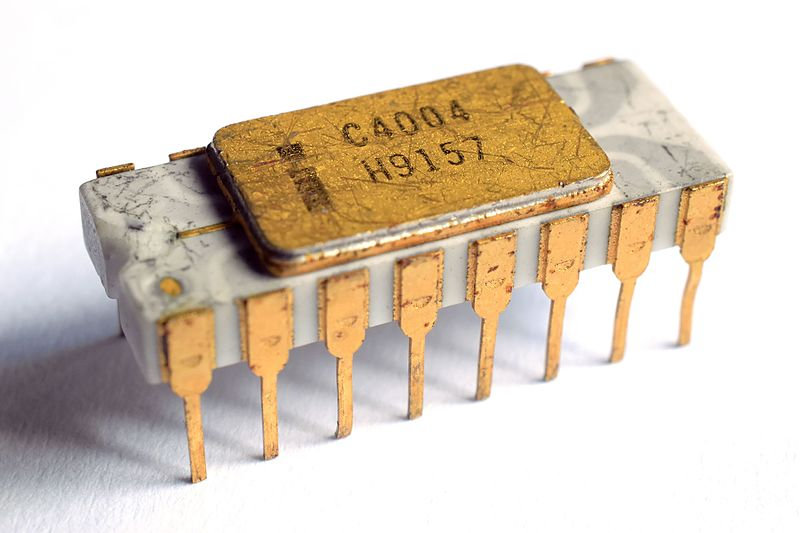
\includegraphics[width=.3\linewidth]{pics/intel_4004} 
\end{center} 
\caption{Intel 4004 microprocessor, an entire CPU on a single chip; the first microprocessor. Released in 1971.\\ \textit{\small{Picture courtesy of Thomas Nguyen}}}
\label{Intel4004}
\end{figure} 

It seems a tipping point had now been reached, the manufacturing cost of computers was low enough, their size was small enough and their performance was high enough that some manufacturers decided to start designing and marketing them to personal users. In 1974, MITS released what can be considered the first market-successful home computer 
\cite{RN41}, the Altair 8800, which used an 8080 microprocessor and is shown in Figure \ref{Altair8800}.

\begin{figure} \begin{center}
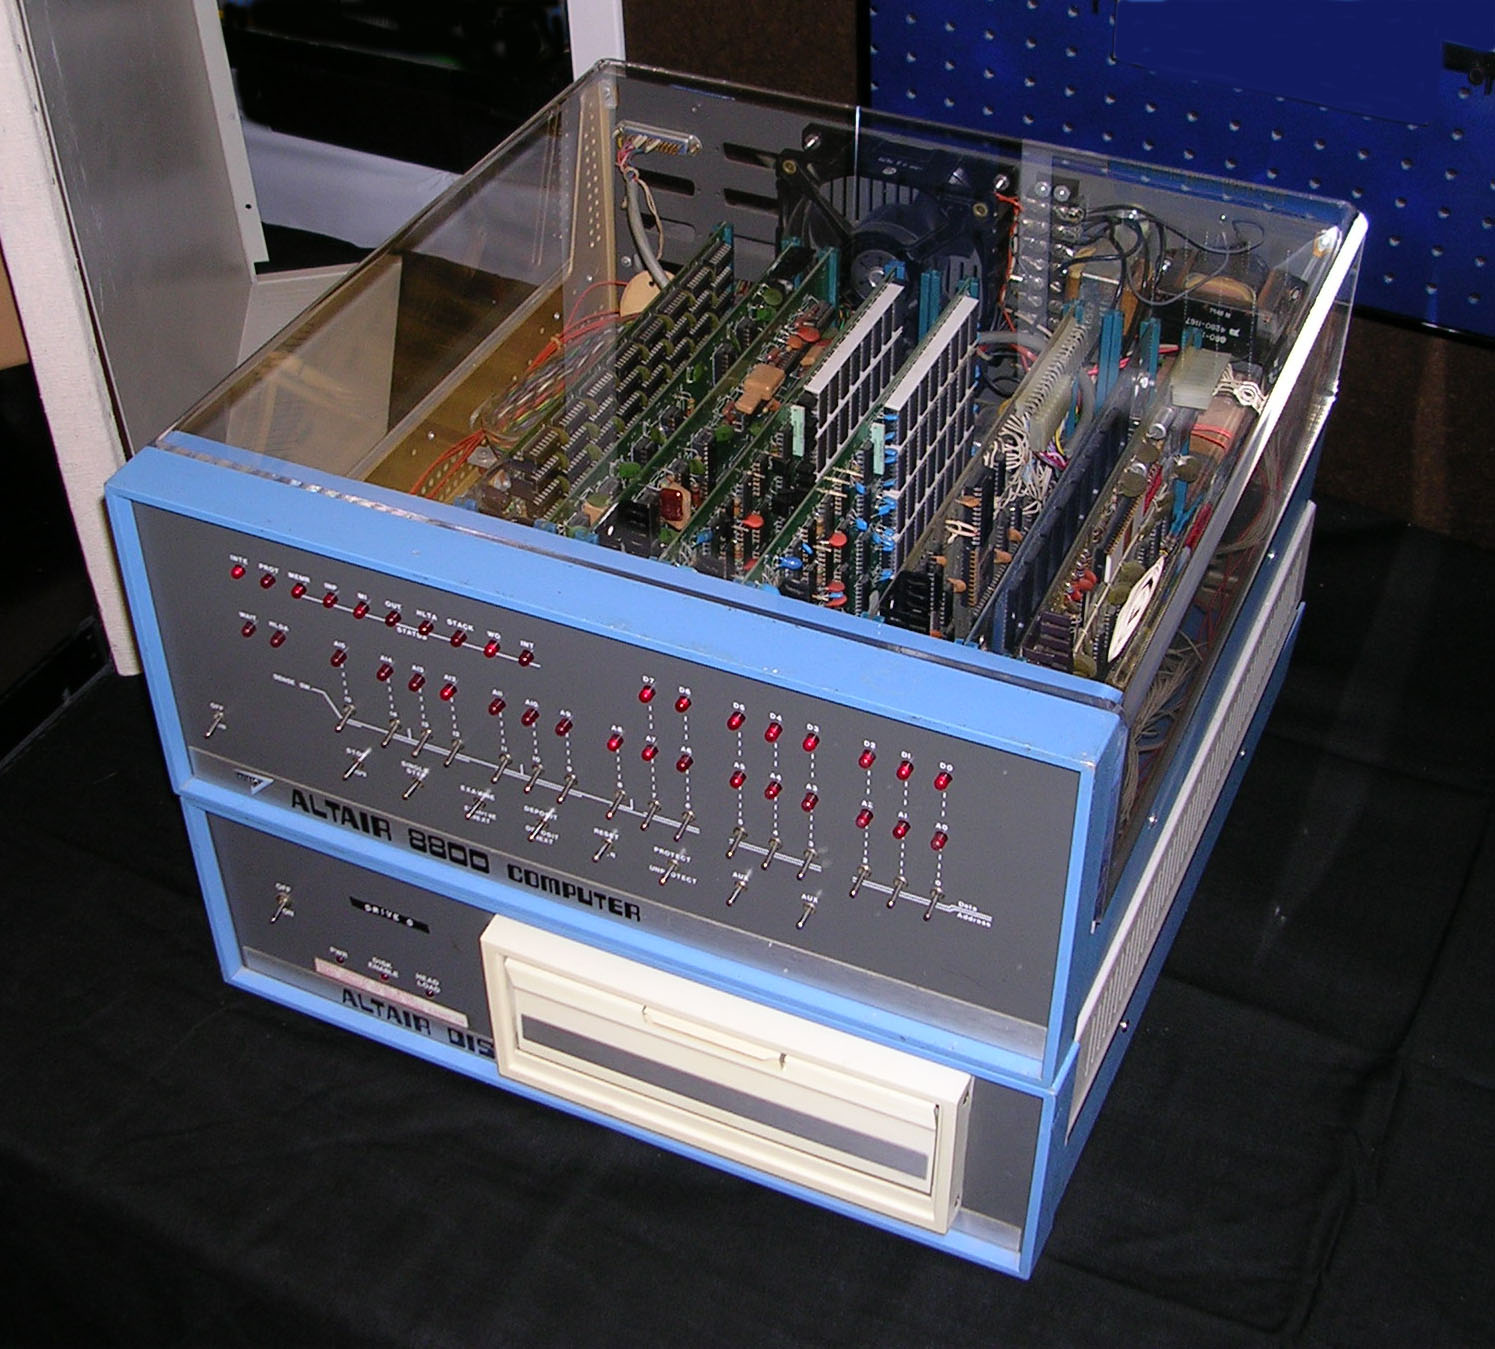
\includegraphics[width=.3\linewidth]{pics/altair_8800_computer} 
\end{center} 
\caption{MITS Altair 8800 home computer, the first market successful home computer. It used an 8-bit 8080 microprocessor and was released in 1974.\\ \textit{\small{Picture courtesy of Michael Holley}}}
\label{Altair8800}
\end{figure}

Over the next 15 or so years, a flurry of new companies sprung up offering a multitude of personal computers 
\cite{RN27}. In the same period new microprocessors where developed, further increasing their performance and new processes where developed that reduced their cost to manufacture. The most notably of these new microprocessors is the 8-bit 6502 by MOS Technology, which when released in 1975 was the least expensive microprocessor on the market by a sizeable margin 
\cite{RN40}. A sense of excitement and seemingly an expectation that computers where going to revolutionise society was abound at this time 
\cite{RN34}. Many people were having their first interactions with computers, as the home computer became more wide spread.

These early home computers had a relatively simple interface compared to modern computers. This meant there was far less abstraction between the user and the inner workings of the computer, this may have allowed their users to more readily understand the underlying mechanisms. It also meant that users had to learn at least some rudimentary programming skills to use them. Another way users where exposed to programming was from the possibility to acquire programs by typing them into their own computers out of magazines or from computer shows on TV and thus exposing them to source code. Most of the home computers in this period ran some form of BASIC, which is a family of general-purpose high-level programming languages, all derived from the original BASIC language created at Dartmouth College in 1964
\cite{RN130}. 

There were some people that questioned the usefulness of the early home computers, and with some merit, as there was a lack of software and distribution channels at the beginning of the era
\cite{RN23}. Others had unrealistic expectations of what computers would do for them, including doing tasks such as putting the rubbish out and babysitting. Home computers where mainly used in a four areas: business, science and engineering, education and in the home. Business, science and engineering uses included spreadsheets, word processing, basic graphics, databases and communication to connect to host computer or LANs. In the home the most widely reaching use of home computers was to play games 
\cite{RN24}. These 8-bit home computers were where many people first met and became interested in the potential of computers and computer programming and they helped kick off a revolution.


%----------------------------------------------------------------------------------------
%----------------------------------------------------------------------------------------
\section{Commodore 64, 128, 65}
\subsection{Commodore 64}
The Commodore 64 (C64) was one of the most successful home computers, selling over 17 million units according to Commodore International 
\cite{RN42}, the now defunct manufacturers of the Commodore 64. Earning it a Guinness World Record (formally Guinness Book of Records): 'Most computer sales'
\cite{RN43}.
It was first sold in January, 1982, for \$595 USD at launch 
\cite{RN28}. The computational power came from a 8-bit MOS Technology 6510 microprocessor, a modified version of the 6502 mentioned in section \ref{sec: Early home computer era}. It had 64 kilobytes of RAM, which was the inspiration of its name. The Commodore 64 was a dominant market presence; in a category of influential home computers, the Commodore 64 may well have been the most influential of all. It ran a version of BASIC and there was a huge software library created for it during its lifetime and there's still new software being developed for the C64 to this day.
\cite{RN82}\cite{RN83}\cite{RN84}.

\subsection{Commodore 128}
The Commodore 128 (C128) was Commodore International's evolution of the very successful Commodore 64. Released in January, 1985, It was meant to build on the success of the C64 while still being near 100\% compatible with Commodore 64 software. It was powered by a more powerful 8-bit 8502 microprocessor and had 128 kilobytes of RAM. An innovation was the inclusion of a second microprocessor, an 8-bit Zilog Z80. This second CPU allowed the C128 to run the CP/M operating system as well as the Commodore BASIC environment similar to the C64. Running CP/M allowed the C128 to access the CP/M software library, which was quite extensive. That coupled with the Commodore 64 software library gave the C128 one of the broadest range of software compared to its competitors of the day
\cite{RN32}.

\subsection{Commodore 65}
The Commodore 65 (C65) was in development in 1990-1991, when Commodore Business Machines (subsidiary of Commodore Intentional) went bankrupt in 1994. In the fallout of the collapse, a number of C65 prototypes where sold and are now a rare and valuable collectors item \cite{RN132}. The C65 was planned to be an upgrade of the C64. \textit{Compute! Gazette} reported in an article in 1989 that the C65 had a 16-bit 65816 microprocessor; a 16-bit version of the 6502 
\cite{RN31}. Years later, when the prototypes where sold on the market by liquidators, sources report a modified 65CE02 microprocessor was used instead
\cite{RN30}
\cite{RN78}. The 65CE02 was an 8-bit CPU with a limited ability to use 16-bit instructions. It had 128 kilobytes of RAM, expandable to 1 megabyte. The C65 had a "stunning" 640x400 pixel maximum resolution 
\cite{RN31} powered by a VIC-III graphics chip. It had a C64 compatibility mode, meant to allow near 100\% compatibility with the C64, but the existing prototypes have significant compatibility problems
\cite{RN30}. 

%----------------------------------------------------------------------------------------
%----------------------------------------------------------------------------------------
\section{History of the MEGA65 project}
\label{History of the MEGA65 project}
Started in December 2013 by Dr. Paul Gardner-Stephen 
\cite{RN44}, the MEGA65 project is attempting to innovate the Commodore 65, with near 100\% compatibility with C64 software. Dr. Gardner-Stephen owned a Commodore 65 prototype between 1994-2010, he also owned a Commodore 128 through the same time and when compared, preferred the C65. Dr. Gardner-Stephen also loved to tinker with these computers during the 1990 and 2000s, devising ways of accelerating the C64 CPU as an example. After deciding to sell the C65 prototype to a collector, Dr. Gardner-Stephen always had the idea of recreating the C65, and implementing some of the tricks and ideas he had worked out or heard of over the years. Then, during Dr. Gardner-Stephen's Ph.D studies, he learnt to program in VHDL and it seemed possible to realise this dream using the technology of FPGAs.

This dream was delayed due to technological issues with the FPGA boards of the time not quite being fast enough for Dr. Gardner-Stephen's vision. But by 2013, a sufficiently powerful and affordable board had been released to the market. Dr. Gardner-Stephen chose a Nexys4 development board, used by a lot of teaching institutions and designed with students in mind. This FPGA has many built in peripherals which can be used by the computer as well as its cost to performance ratio makes it ideal. The added benefit of using off-the-shelf FPGA board is that availability should be much greater compared to a PCB created just for MEGA65, which would be limited to small production runs carried out by the MEGA65 team or others using the open-source designs 
\cite{RN45}.

The MEGA65 project is completely open-source with the hardware VHDL/verilog files describing the hardware and operating system software available on a public git repository 
\cite{RN17}. Dr. Gardner-Stephen's stated goals at the inception of the MEGA65 project were as follows \cite{RN45}:

\begin{itemize}[before=\itshape]
\item Better graphics than the Apple IIgs, Atari 800 or Plus/4: 1920x1200 @ 60Hz, 256 colour palette from 4,096 colours (later from 24-bit colour palette once I create an HDMI output) via my VIC-IV video controller.
 \item    Better sprites than the C64.  Plan is for the 8 compatibility sprites, plus perhaps 32 256-colour Enhanced Sprites with hardware scaling and practically unlimited size.  Maximum number of displayable sprites will depend on the resolution of the display and the sprites on a given raster line.
 \item    Faster CPU than the SuperCPU or any available 65C816 CPU (20MHz), and ideally with enough headroom to beat a 20MHz 65C816 running in 16-bit mode.  Currently the 65GS10 runs at 96MHz, but with an effective speed more like 48MHz until I work on some planned IPC improvements, like a 16-bit cache of zero-page to make zero-page indirect instructions take as little as 3 cycles.
 \item    More RAM than a fully expanded Apple IIgs or C65 (~8.125MB).  It will initially have 128KB of chipram like the C65, plus 16MB of slowram, plus "some" ROM.
 \item    Comparable or better sound capability than the Apple IIgs.  Multiple SIDs plus digital audio channels.  Design to be finalised.
 \end{itemize}  

  
After discussions to make sure their goals where aligned, In April 2015, Dr. Gardner-Stephen and the Museum of Electronic Games and Art (MEGA) announced a partnership to make an open-source Commodore 65-like computer 
\cite{RN47}, called the MEGA65. When asked about the motivation of the project in the press, Dr. Gardner-Stephen remarked "While It is \textit{rather} pointless, it isn't \textit{completely} pointless. It's like the difference between mostly dead and completely dead in The Princess Bride.  The MEGA65 will be fun for those for whom it is fun, which is one purpose.  Also, I intend to build and use a set of MEGA65 computers in teaching" 
\cite{RN48}.

The core of  the MEGA65, which provides the computational power, comes from a innovation of a 4502 microprocessor design; the 45GS02.
In 2015 there where plans for a laptop as well as a C65-like form factor for the MEGA65, but during development the plans changed to replace the laptop with a smart phone form factor. Several other people besides Dr. Gardner-Stephen have also started working on this project including open-source community members, Flinders University students and staff. 

During development Dr. Gardner-Stephen also conceived of another potential use for the MEGA65, as a secure device for communication and general computing. This is thought possible by leveraging a characteristic of the MEGA65: simplicity, both in its hardware and software. This along with its open-source nature, allows the MEGA65 to be completely verifiable that it is secure. Some extra features have been added to facilitate a secure device, which is talked about in Chapter \ref{Chapter5}. The MEGA65 is currently in a prototype phase of development.

%----------------------------------------------------------------------------------------
%----------------------------------------------------------------------------------------
\section{The progressing complexity of computer hardware and software}
\label{The progressing complexity of computer hardware and software}
The story of complexity and computers starts very much the same as the story of home computers. The technological advances led to ICs being smaller, faster, cheaper and more complex. Computer manufacturers also started using more ICs in their computers, further increasing the complexity. At the same time, software for computers has been increasingly getting more complex. 

\subsection{History of CPU complexity}
An informed discussion on complexity in computer hardware cannot be made without mention of Moore's Law. Gordan Earle Moore, Northern American engineer and co-founder of Intel Corporation, wrote a seminal paper in 1965 titled \textit{Cramming More Components onto Integrated Circuits}. In this paper he observed a trend in electronics: ICs are the future of electronics and they have been getting small, faster and cheaper
\cite{RN33}. He also predicted this trend would continue into 1975, and predicted the advances in ICs would power new technologies such as home computers, automatic controls for cars and 'person portable communication equipment' or mobile phones 
\cite{RN33}. In 1975, Moore wrote another paper, \textit{Progress In Digital Integrated Electronics}, revisiting his earlier prediction. In this paper he observed 'Complexity of integrated circuits has approximately doubled every year since their introduction' 
\cite{RN52}. He also predicted this would continue into the future and it largely has, as seen in Figure \ref{tran_count_over_time}. 

\begin{figure} \begin{center}
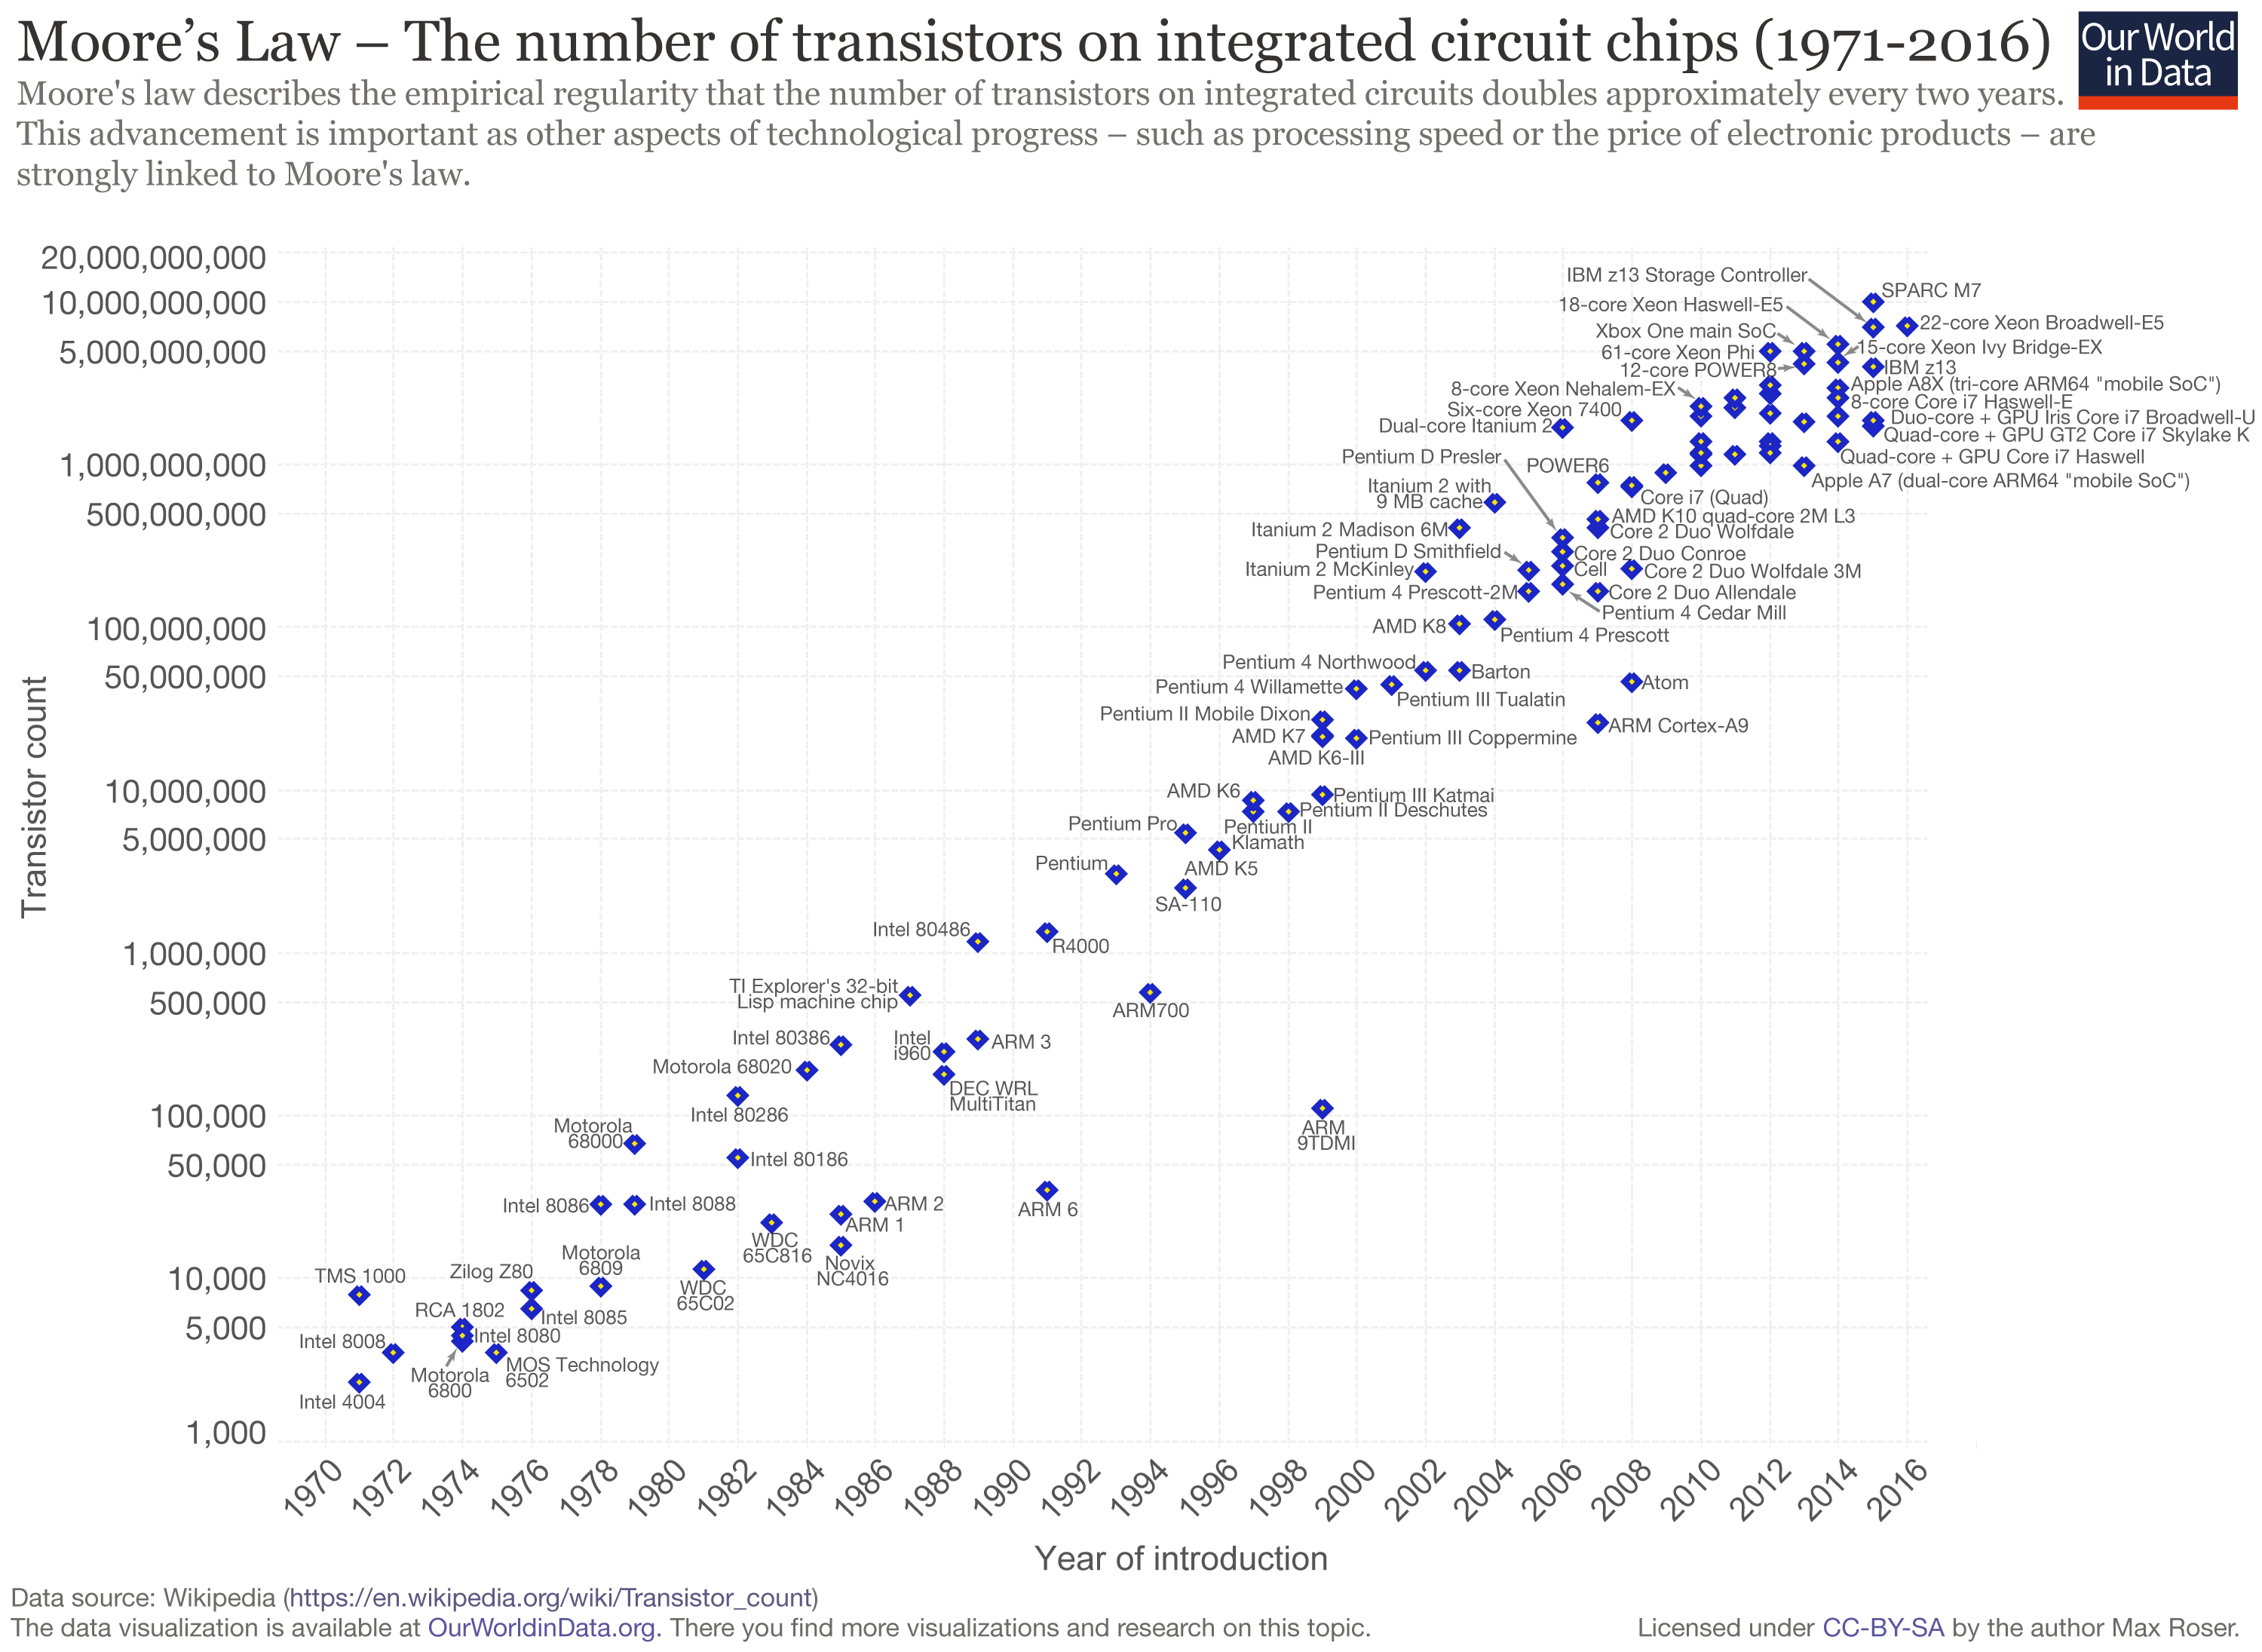
\includegraphics[width=1\linewidth]{pics/moore_law} 
\end{center} 
\caption{Plot of transistor count vs released year for microprocessors\\ \textit{\small{Picture courtesy of Max Roser}}}
\label{tran_count_over_time}
\end{figure}

So it can been seen that transistor count has increased almost in line with Moore's prediction, with some modern CPUs having upwards of 19 billion transistors 
\cite{RN80}. But is an increase in transistor count related to an increase in complexity? Yes, they are directly proportional; by the very definition of complexity, adding more transistors to an IC would increase its complexity. 

For the last few years it has become apparent that the amount of performance increase from each new generation of ICs is not as large as previously. This is due to physical limitations; the silicon wafers are merely nanometres wide already, so they simply cannot be made much smaller
\cite{RN141}. There are also physical limitations in the amount of heat dissipation that can be achieved as well as problems with current leakage. These problems have led to some speculation that Moore's law could be reaching an end 
\cite{RN49}.

\subsection{History of operating systems complexity}

Software, like hardware, has also been growing increasingly complex, driven by a demand that is growing faster than our capacity to design, test, implement and maintain it
\cite{RN85}. Many people have remarked on the steady increase in software complexity and the adverse effects it has on security, maintenance and design costs. Bruce Shneider has written extensively on computer security topics and successfully argues that 'complexity is the enemy of security' 
\cite{RN11} \cite{RN3}. Edward Ogheneovo wrote and interesting paper linking increased complexity to increased maintenance costs for software 
\cite{RN81}. Lawson takes a broader view, talking about the complexity of computer systems as a whole and how software affects that complexity 
\cite{RN55}, as well as the rise in complexity over time. Gelsinger et al. talks about the increase in software complexity driven by the need to keep up with rapid hardware changes while designing microprocessors at Intel 
\cite{RN18}. These papers are discussed more in section \ref{subsec: Complexity as the root cause of modern malware susceptibility} but the salient point linking them is that software complexity is increasing. To further argue this point, a comparison of different versions of popular operating systems is made, as seen in Figure \ref{SLOC_windows} and Figure \ref{SLOC_linux}. These graphs compare the Source Lines Of Code (SLOC) which is the number of lines of code in the source code before it's compiled. Other metrics were considered, such as the cyclomatic complexity of the source code or the permanent memory space required to install the software. But the availability of the cyclomatic complexity data was lacking and the SLOC was determined to be a more accurate indicator of complexity than the installation size of an operating system. This is partly due to the fact that installation size could be bloated with elements that are not that complex but require a large amount of memory space, such as video, bitmap and audio files. The reason operating systems where considered the best type of software to compare is that they (at least the versions chosen for comparison) are designed for home computers or their modern equivalents and have been is use from the early home computer era until now. 

\begin{figure} \begin{center}
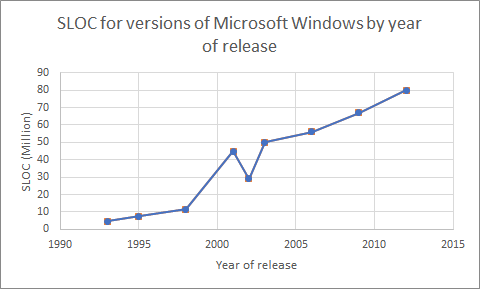
\includegraphics[width=0.8\linewidth]{pics/SLOC_windows} 
\end{center} 
\caption{Source Lines Of Code (SLOC) for different version of Windows operating system vs released year\\ \textit{\small{Data provided by \cite{RN81}}}}
\label{SLOC_windows}
\end{figure}

\begin{figure} \begin{center}
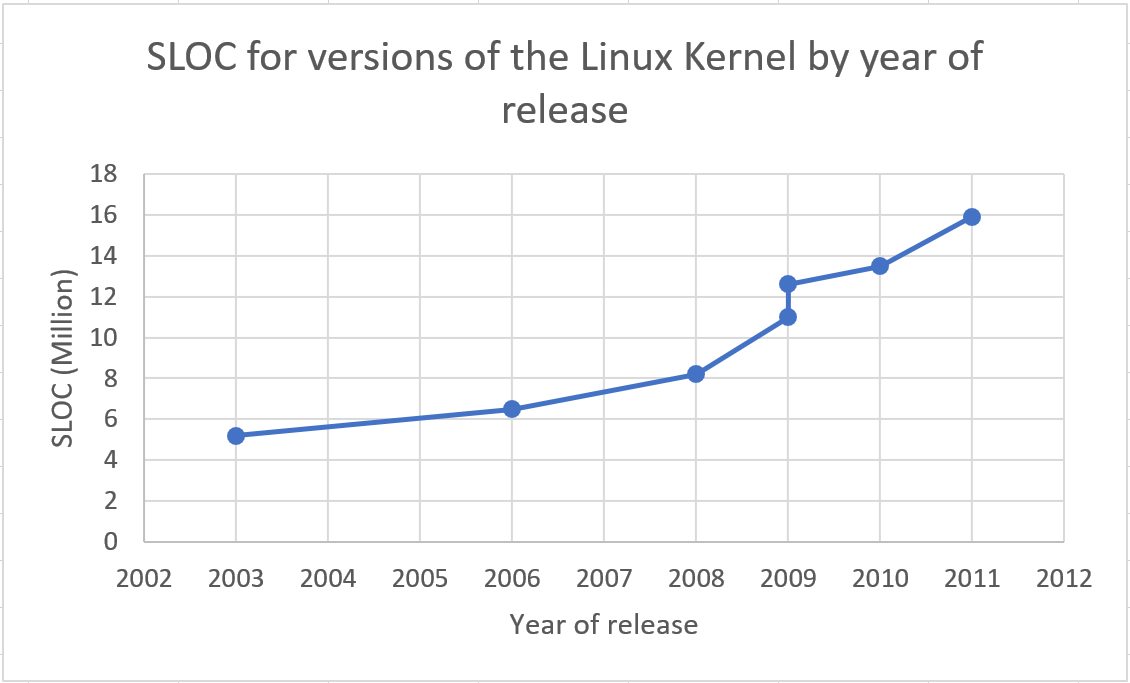
\includegraphics[width=0.8\linewidth]{pics/SLOC_linux} 
\end{center} 
\caption{Source Lines Of Code (SLOC) for different version of the Linux Kernel vs released year\\ \textit{\small{Data provided by \cite{RN81}}}}
\label{SLOC_linux}
\end{figure}

%----------------------------------------------------------------------------------------
%----------------------------------------------------------------------------------------
\section{History of computer insecurity}
\label{History of computer insecurity}
Security is described in \textit{RFC4949 Internet Security Glossary, Version 2} as a system condition where system resources are free from unauthorised access 
\cite{RN66}. In recent years computer security has been a widely discussed topic, mainly due to the damage that malicious programs, or malware, have caused. There are several Standards dealing just with this issue, which shows its importance in modern business and engineering 
\cite{RN70}\cite{RN68}\cite{RN69}. It is now common for companies to lose more from electronic theft than it is from physical theft 
\cite{RN76}. This was not always the case. It seems the inevitable fate of any new successful technology, to be manipulated by malicious actors. Computers and self-reproducing virus programs are both technologies which befell this fate.

Computer security had an interesting beginning. The terms we use today had not be ‘coined’ or where not in common usage, or even are used to mean something slightly different than they do now, such as the computer virus. So to begin, a brief discussion of the origin of some common (by today's standard) phrases.

\textbf{Bug/Debugging:} In 1947 Rear Admiral Grace Murray Hopper noticed the Mark II computer she was using was outputting unexpected results and upon inspection found a moth across a relay, shorting it out 
\cite{RN75}. While the term bug was used in electrical engineering fields, this event is credited with popularising the terms use with computer programmers. A computer system ‘bug’ is an unexpected system behaviour. In this case the relay was shorted out, causing some unexpected behaviour. 

\textbf{Virus:} Fred Cohen first uses the term in his Ph.D. paper, \textit{Computer viruses: Theory and experiments}, published in 1987. 
\cite{RN61}. It followed on from Jon Neuman’s seminal work on self-reproducing automata, Cohen describes a virus as "a program that can ‘infect’ other programs by modifying them to include a possibly evolved copy of itself" \cite{RN61}. Cohen also establishes viruses as a morally neutral technology; meaning it could be employed for good or bad deeds. Cohen mentions several beneficial uses for viruses in the paper, as well as security concern relating to viruses \cite{RN61}. The name virus comes from the fact that the program behaves similar to a biological virus, as it must attach itself to another program, similar to a biological virus attaching itself to another cell. In the time since Cohen's definition, the meaning of a computer virus has changed to mean almost exclusively a form of malware. This change in definition has been encouraged by anti-virus companies, in a bid to help sell their products 
\cite{RN64}. 

\textbf{Worm:} Similar to a virus in that it is a self-reproducing program, the difference come in the fact a worm can execute by itself where as a virus has to attach to another piece of software. Also similar to viruses in that worms are now almost always malware but they first appeared as beneficial programs \cite{RN93}.

\textbf{Malware:} A portmanteau of malicious and software, which aptly describes malware; it is malicious software designed to cause harm. Examples of malware used today are Trojan Horses, Logic Bombs, Key-loggers, Lures, Worms and Viruses.

\textbf{Ransomware:} Also known as a cryptovirus or a cryptoworm. It is another type of malware which encrypts sensitive information and demands payment from the victim to decrypt the data. Payment is normally asked for in e-money such as Bitcoin because it is much harder to trace.
\\

As computer systems have gradually been used to control and store more and more vital information and services, so have the efforts of malicious parties to break into these computer systems for their own benefit. In 1964, AT\& T, a Northern American telecommunications company started monitoring phone calls to catch people illegally using their phone lines to make long distance phone calls for free. This practise involved the use of devices to imitate the tones used by AT\& T to control their phone system. These devices could be an electronic tone generator, a version of which is seen in Figure \ref{blue_box} or simply a cassette tape recording of keyboard notes
\cite{RN56}. 1970 saw the first worms created at Xerox's Palo Alto Research Centre. A series of benevolent worms where created to carry out a variety of useful task, such as display messages or use a computer for calculations when it would otherwise be idle. Due to an error, one of these worm programs misbehaved and caused every computer infected with it to crash and on re-starting the computer it would be re-infected and crash immediately 
\cite{RN93}. This event proved the potential for worms to cause massive damage to computer systems and afterwards public research was lacking for several years but it almost certainly continued in secret. In 1986, the Brain virus was found on infected computers in North America. It was designed by two brothers in Pakistan who ran a computer shop, they where worried about pirated copies of their programs and devised the Brain virus as a way to fix this problem. Once infected, a computer would display a message letting the user know they are using pirated software and gave the contact details of the brother's computer shop to get a 'vaccination' 
\cite{RN86}. Worms re-emerged into the public spotlight in 1988 with the now infamous Morris Worm, thought to have infected 10\% of the 60,000 computers predicted to be connected to the internet at the time. It achieved wide spread news coverage becoming infamous. Released on November 2, 1988, the Morris worm effectively brought the internet to a stand still 
\cite{RN90}. There where numerous other worms and viruses created around the same time. These early incidents raised awareness of malware and computer security. Several anti-virus companies formed after these events.

Since the first malware was created, the problem has simple grown. With more and more computer systems controlling important information around the world, the incentive for malicious actors to break into them has grown. As more and more people use computer systems to communicate and organise their daily activities, the incentive for malicious actors to try and deceive people into divulging sensitive information increases. There are now daily reports of malware attacks as well as sophisticated scams run entirely online. While some scams don't involve any malware, but may be simply a deceitful email asking for sensitive information, the definition of security used above is broad enough to cover these cases too. Governments of many countries now employ computer security experts to help protect themselves, as well as developing malware to use against their adversaries. A well known example of a  government-made malware is the Stuxnet virus. Stuxnet was found on an infected computer in 2010 by Sergey Ulasen. Ulasen ran a small computer security firm and a client was seeking help with a computer stuck in a reboot loop. This triggered a massive investigation by several companies which lead to the conclusion that Stuxnet was a targeted malware designed to hinder Iran's nuclear enrichment capabilities. The target as well as the amount of effort that went into Stuxnet, lead many to believe it must have been a state-sponsored malware attack, with Israel and the USA being the most likely culprits 
\cite{RN91}\cite{RN92}. The Stuxnet virus was also interesting because it was the first case of a malware 'in the wild' being used to cause physical damage, where as the harm caused by other malware seen before it was limited to computer systems. Stuxnet virus was designed to attack PLC controllers connected to frequency converter drives in one specific nuclear enrichment plant in Iran. Once these PLCs were identified, Stuxnet would then routinely run the drives at frequencies that would cause them to break. There are many, many, many more examples of malware and computer security issues, with more happening each day. Its worth noting that there has been a general trend of malware being used to steal money, the first malware seemed to have been created out of curiosity and now more often than not malware is being used to steal money or valuable information which can be sold to other criminals. The WannaCry ransomware being a salient recent example of modern malware being created to steal money 
\cite{RN94}. 

\begin{figure} \begin{center}
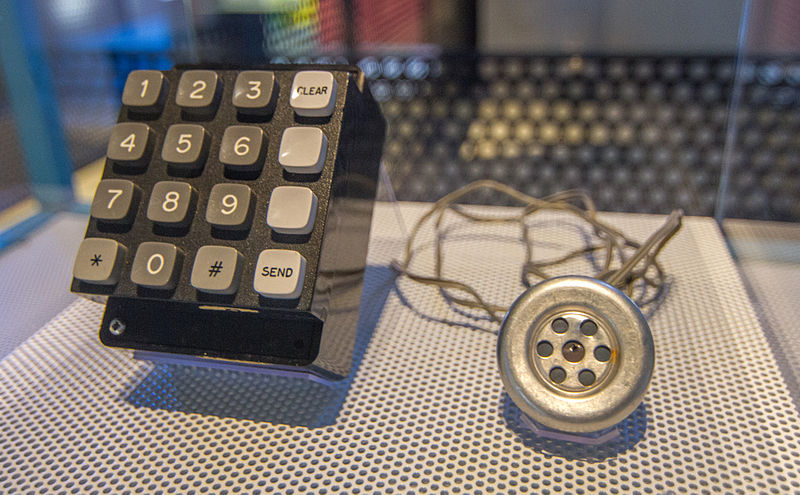
\includegraphics[width=0.8\linewidth]{pics/blue_box} 
\end{center} 
\caption{A Blue Box; electronic tone generating device used to gain access to AT\& T's phone network in North America\\ \textit{\small{Picture courtesy of Maksym Kozlenko}}}
\label{blue_box}
\end{figure}


\subsection{Complexity is the root cause of modern malware susceptibility} 
\label{subsec: Complexity as the root cause of modern malware susceptibility}
There is one common aspect linking each and every case of computer security being breached, they all use some vulnerability within the computer system (the system being inclusive of the users) to gain access they shouldn't have. These vulnerabilities can be in the software, hardware or even in the users choice or password or their habits (use of USB drives, physical security of their computer etc.). In the examples listed in section \ref{History of computer insecurity}, AT\& T had a vulnerability in their phone system in that anyone could control the system through the use of tones played down the line. It can be guessed that the idea that malicious actors would attempt do this this was not considered likely or considered at all when the system was first designed. The Brain virus exploited vulnerability found in MS-DOS operating system, which was new at the time \cite{RN86}. The Morris worm exploited weak passwords as well as vulnerability with in Unix's sendmail, fingerd and rsh/rexec commands 
\cite{RN86}. Stuxnet exploited four zero-day vulnerabilities, which is unprecedented and one of the reasons it is believed to be a state-sponsored malware\cite{RN91}. A zero-day vulnerabilities is a vulnerabilities that is not publicly known; the software manufacture is unaware of it. WannaCry exploited a flaw in the Windows operating system \cite{RN94}. So it can be concluded that malware needs a vulnerability to exploit if it is going to gain unauthorised access to a computer system. So what is a vulnerabilities?, what causes them? and how can they be avoided? These are all logical questions that follow. 

A vulnerability can be described as a way to let unauthorised actors enter a computer system, which is perhaps not that illuminating in terms of explaining what it is. This is because vulnerabilities can have so many forms, ranging from hardware design flaws such as the type that caused the Meltdown and Spectre exploits to be possible \cite{RN16}, to software flaws such as the type exploited by Stuxnet and WannaCry \cite{RN91}\cite{RN94}. There could be vulnerabilities in the users selection of password, as exploited in the Morris worm \cite{RN86}. Users can also provide other vulnerabilities in there use of external media they connect to the computer system as well as the physical security of devices connected to the computer system. This was the case with Stuxnet, as it is believed to have entered the target computer network from a USB storage device, as the computer network in question was isolated from the internet \cite{RN91}. So vulnerabilities are varied and many in their forms, but what causes them? and how can they be avoided?

So vulnerabilities are way to access a computer network through means that shouldn't be possible in a ideal world. And it follows that these vulnerabilities are only possible if they are never found or thought of by the designers and/or manufacturers and then fixed. So what would make it hard for the designers to find the aforementioned vulnerabilities? Well, if the task is simply too large, the design so complex, it's simply too hard to consider every possible avenue of access into the computer system. As talked about earlier in section \ref{The progressing complexity of computer hardware and software}, software and hardware have both been continually getting more complex to meet our demand for more functionality, power and convenience. This complexity will almost certainly lead to more vulnerabilities.

Bruce Shneider has extensively talked about what he calls a truism; that "complexity is the worst enemy of security" \cite{RN96}. Scheider first mentioned this in 1999, in his security blog \cite{RN3} and has since talked about it in at least two of his books \textit{Secrets and Lies} (2000) and \textit{Practical Cryptography} (2003) as well as in various articles and interviews. Shneider convincingly argues that good security come from getting everything right: careful analysis of source code, specifications and systems. A more complex system will require more detailed and expensive analysis, with greater chance of a vulnerability being overlooked, as there is simply more to look at. The more complex a system is: the more lines of codes make up said system, the more interactions with other systems it has, the more configuration options available and the more vulnerabilities there are. With a complex system there is more to get wrong and good security require that everything is done correctly.

Edward E. Ogheneovo wrote an illuminating paper titled \textit{On the Relationship between Software
Complexity and Maintenance Costs} in 2014. In the paper he claims software is increasing in complexity and an increase in complexity drives up the cost of maintaining the software. He successfully links  maintenance costs to the amount of bugs in the software and shows that the root cause of the bugs is complexity \cite{RN81}. 

While working at Intel during the turbulent 1980's to 2010, Patrick Gelsinger, Desmond Kirkpatrick,
Avinoam Kolodny, and Gadi Singer witnessed first-hand the increase in complexity, both in hardware being designed by themselves as well as the CAD software created to facilitate the design process. They provide an excellent recounting of this period at Intel in the paper \textit{Such a CAD!}. They illustrate clearly what is driving this increase in complexity: demand \cite{RN18}. Customers demand and expect more powerful computer products in line with Moore's Law, this is not to say most customers where aware of Moore's Law, but they where aware (within a few years of the home computer era) that computers continually got more powerful. If Intel didn't meet this demand, others would have and Intel would not have been as successful in business.

Going back to 1987 and Fred Cohen's seminal paper \textit{Computer viruses: Theory and experiments}. Cohen comes to the conclusion that the sharing of information needed in a general purpose computer, such as a home computer or PC, is in direct opposition to the goals of viral security. Which is implying that computer systems where are already becoming too complex in relation to viral security in 1987.

With all this in mind, it can be said that the root cause of malware susceptibility and computer insecurity is complexity. Which leaves the question, what can be done about it? This question is beyond the scope of this thesis but a possible answer is given in in section \ref{History of the MEGA65 project}, an open-source simple computer.
